\documentclass[tikz,border=2pt]{standalone}
\usetikzlibrary{arrows.meta,automata,positioning}
\usepackage{siunitx}
\definecolor{celadon}{rgb}{0.67, 0.88, 0.69}
\definecolor{lightskyblue}{rgb}{0.61, 0.87, 1.0}
\definecolor{bluebell}{rgb}{0.64, 0.64, 0.82}

\begin{document}
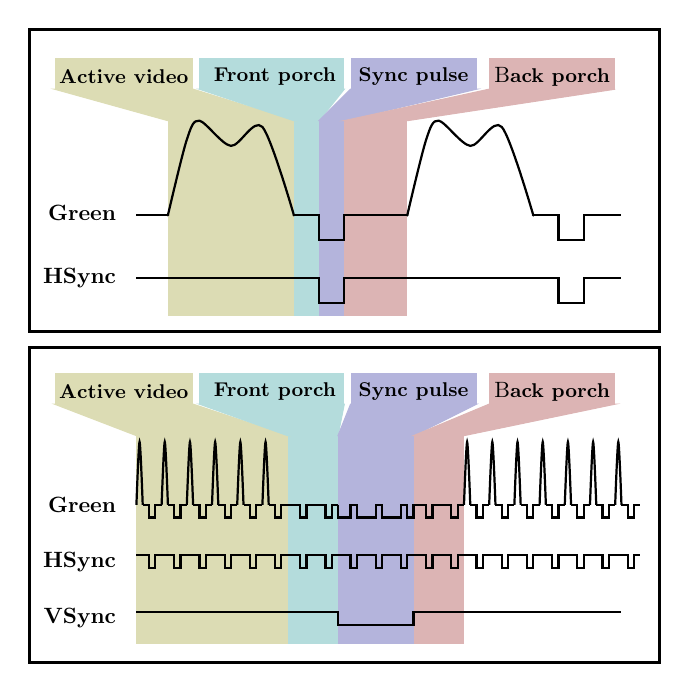
\begin{tikzpicture}[scale=0.8, transform shape]
\definecolor{active}{RGB}{220,220,180}
\definecolor{front}{RGB}{180,220,220}
\definecolor{sync}{RGB}{180,180,220}
\definecolor{back}{RGB}{220,180,180}

% ======================================================
% SCHEMA 1 (sopra)
% ======================================================

%cornice
\node[rectangle,
    draw,
    very thick,
    minimum width = 10cm, 
    minimum height = 4.8cm] (a) at (0,2.55) {};

% colori
\fill[active] (-2.8,0.4) rectangle (-0.8,3.5);
\fill[front]  (-0.8,0.4) rectangle (-0.4,3.5);
\fill[sync]   (-0.4,0.4) rectangle (0,3.5);
\fill[back]   (0,0.4) rectangle (1,3.5);

\filldraw[fill=active, draw=active]
  (-2.8,3.5) -- (-0.8,3.5) -- (-2.4,4) -- (-4.6,4) -- cycle;
\filldraw[fill=front, draw=front]
  (-0.8,3.5) -- (-0.4,3.5) -- (0,4) -- (-2.3,4) -- cycle;
\filldraw[fill=sync, draw=sync]
  (-0.4,3.5) -- (0,3.5) -- (2.1,4) -- (0.1,4) -- cycle;
\filldraw[fill=back, draw=back]
  (0,3.5) -- (1,3.5) -- (4.3,4) -- (2.3,4) -- cycle;

\fill[active] (-4.6,4) rectangle (-2.4,4.5);
\fill[front]  (-2.3,4) rectangle (0,4.5);
\fill[sync]   (0.1,4) rectangle (2.1,4.5);
\fill[back]   (2.3,4) rectangle (4.3,4.5);

% Titoli sezioni
\node at (-3.5,4.2) {\small \textbf{Active video}};
\node at (-1.1,4.2) {\small \textbf{Front porch}};
\node at (1.1,4.2) {\small \textbf{Sync pulse}};
\node at (3.3,4.2) {B\small \textbf{ack porch}};

% Etichette
\node[left] at (-3.5,2.04) {\textbf{Green}};
\node[left] at (-3.5,1) {\textbf{HSync}};

% Green (analogico)
\draw[thick]
plot[smooth] coordinates {
(-2.8,2)
(-2.5,3.2)
(-2.3,3.5)
(-1.8,3.1)
(-1.3,3.4)
(-0.8,2)
};
\draw [fill] (-2.8,2) circle [radius=0.01];
\draw [fill] (-0.8,2) circle [radius=0.01];

\draw[thick]
plot coordinates {
(-3.3,2)
(-2.8,2)
};

\draw[thick]
plot coordinates {
(-0.8,2)
(-0.4,2)
(-0.4,1.6)
(0,1.6)
(0,2)
(1,2)
};

\draw[thick]
plot[smooth] coordinates {
(-2.8+3.8,2)
(-2.5+3.8,3.2)
(-2.3+3.8,3.5)
(-1.8+3.8,3.1)
(-1.3+3.8,3.4)
(-0.8+3.8,2)
};
\draw [fill] (-2.8+3.8,2) circle [radius=0.01];
\draw [fill] (-0.8+3.8,2) circle [radius=0.01];

\draw[thick]
plot coordinates {
(-3.3+3.8,2)
(-2.8+3.8,2)
};

\draw[thick]
plot coordinates {
(-0.8+3.8,2)
(-0.4+3.8,2)
(-0.4+3.8,1.6)
(0+3.8,1.6)
(0+3.8,2)
(1+3.4,2)
};

% HSync
\draw[thick]
plot coordinates {
(-3.3,2-1)
(-0.4,2-1)
(-0.4,1.6-1)
(0,1.6-1)
(0,2-1)
(1,2-1)
(-0.4+3.8,2-1)
(-0.4+3.8,1.6-1)
(0+3.8,1.6-1)
(0+3.8,2-1)
(1+3.4,2-1)
};

% ======================================================
% SCHEMA 2 (sotto)
% ======================================================

%cornice
\node[rectangle,
    draw,
    very thick,
    minimum width = 10cm, 
    minimum height = 5cm] (a) at (0,-2.6) {};

% colori
\fill[active] (-3.3,0.2-5) rectangle (-0.9,3.5-5);
\fill[front]  (-0.9,0.2-5) rectangle (-0.1,3.5-5);
\fill[sync]   (-0.1,0.2-5) rectangle (1.1,3.5-5);
\fill[back]   (1.1,0.2-5) rectangle (1.9,3.5-5);

\filldraw[fill=active, draw=active]
  (-3.3,3.5-5) -- (-0.9,3.5-5) -- (-2.4,4-5) -- (-4.6,4-5) -- cycle;
\filldraw[fill=front, draw=front]
  (-0.9,3.5-5) -- (-0.1,3.5-5) -- (0,4-5) -- (-2.3,4-5) -- cycle;
\filldraw[fill=sync, draw=sync]
  (-0.1,3.5-5) -- (1.1,3.5-5) -- (2.1,4-5) -- (0.1,4-5) -- cycle;
\filldraw[fill=back, draw=back]
  (1.1,3.5-5) -- (1.9,3.5-5) -- (4.3,4-5) -- (2.3,4-5) -- cycle;

\fill[active] (-4.6,4-5) rectangle (-2.4,4.5-5);
\fill[front]  (-2.3,4-5) rectangle (0,4.5-5);
\fill[sync]   (0.1,4-5) rectangle (2.1,4.5-5);
\fill[back]   (2.3,4-5) rectangle (4.3,4.5-5);

% Titoli sezioni
\node at (-3.5,4.2-5) {\small \textbf{Active video}};
\node at (-1.1,4.2-5) {\small \textbf{Front porch}};
\node at (1.1,4.2-5) {\small \textbf{Sync pulse}};
\node at (3.3,4.2-5) {B\small \textbf{ack porch}};

% Etichette
\node[left] at (-3.5,2.4-5) {\textbf{Green}};
\node[left] at (-3.5,1.5-5) {\textbf{HSync}};
\node[left] at (-3.5,0.6-5) {\textbf{VSync}};

% Green (impulsi)
\foreach \x in {-3.3,-2.9,...,-0.9} {
    \draw[thick]
        plot[smooth] coordinates {
        (\x,2.4-5)
        (\x+0.05,2.4-5+1)
        (\x+0.1,2.4-5)
        };
    \draw[thick]
        plot coordinates {
        (\x+0.1,2.4-5)
        (\x+0.2,2.4-5)
        (\x+0.2,2.4-5-0.2)
        (\x+0.3,2.4-5-0.2)
        (\x+0.3,2.4-5)
        (\x+0.4,2.4-5)
        };
}

\foreach \x in {-0.9,-0.5,...,-0.5} {
    \draw[thick]
        plot coordinates {
        (\x,2.4-5)
        (\x+0.2,2.4-5)
        (\x+0.2,2.4-5-0.2)
        (\x+0.3,2.4-5-0.2)
        (\x+0.3,2.4-5)
        (\x+0.4,2.4-5)
        };
}

\draw[thick]
        plot coordinates {
        (-0.1,2.4-5)
        (-0.1,2.4-5-0.2)
        (0.1,2.4-5-0.2)
        (0.1,2.4-5)
        (0.2,2.4-5)
        (0.2,2.4-5-0.2)
        (0.5,2.4-5-0.2)
        (0.5,2.4-5)
        (0.6,2.4-5)
        (0.6,2.4-5-0.2)
        (0.9,2.4-5-0.2)
        (0.9,2.4-5)
        (1,2.4-5)
        (1,2.4-5-0.2)
        (1.1,2.4-5-0.2)
        (1.1,2.4-5)
        (1.3,2.4-5)
        (1.3,2.4-5-0.2)
        (1.4,2.4-5-0.2)
        (1.4,2.4-5)
        (1.7,2.4-5)
        (1.7,2.4-5-0.2)
        (1.8,2.4-5-0.2)
        (1.8,2.4-5)
        (1.9,2.4-5)
        };

\foreach \x in {1.9,2.3,...,4.4} {
    \draw[thick]
        plot[smooth] coordinates {
        (\x,2.4-5)
        (\x+0.05,2.4-5+1)
        (\x+0.1,2.4-5)
        };
    \draw[thick]
        plot coordinates {
        (\x+0.1,2.4-5)
        (\x+0.2,2.4-5)
        (\x+0.2,2.4-5-0.2)
        (\x+0.3,2.4-5-0.2)
        (\x+0.3,2.4-5)
        (\x+0.4,2.4-5)
        };
}

% hsync
\foreach \x in {-3.3,-2.9,...,4.4} {
    \draw[thick]
        plot coordinates {
        (\x,2.4-5-0.8)
        (\x+0.2,2.4-5-0.8)
        (\x+0.2,2.4-5-0.2-0.8)
        (\x+0.3,2.4-5-0.2-0.8)
        (\x+0.3,2.4-5-0.8)
        (\x+0.4,2.4-5-0.8)
        };
}

% vsync
\draw[thick]
plot coordinates {
(-3.3,2-1-5.3)
(-0.1,2-1-5.3)
(-0.1,2-1-0.2-5.3)
(1.1,1-0.2-5.3)
(1.1,1-5.3)
(1+3.4,1-5.3)
};


\end{tikzpicture}
\end{document}